%versi 2 (8-10-2016)
\chapter{Landasan Teori}
\label{chap:teori}

\section{KIRI Website }
\label{sec:KIRI} 
KIRI adalah aplikasi navigasi angkutan umum berbasis web yang melayani Bandung dan kota-kota lain di Indonesia.\cite{pascal:17:KIRI}.
Pada awal pembuatannya KIRI dibuat untuk tujuan komersial. Namun karena dinilai kurang sukses project KIRI sekarang menjadi open source project yang dapat di akses. Aplikasi KIRI memiliki beberapa fitur sebagai berikut:
\begin{itemize}
    \item Pemilihan rute tercepat menggunakan angkutan kota.
    \item Menampilkan tempat pergantian angkutan kota.
    \item Memiliki fitur multi bahasa.
    \item Memiliki fitur pemilihan lokasi.
    \item Dapat menampilkan beberapa pilihan rute.
    \item Dapat menampilkan instruksi lengkap  mencapai tujuan.
\end{itemize}

\begin{figure}[H]
    \centering
    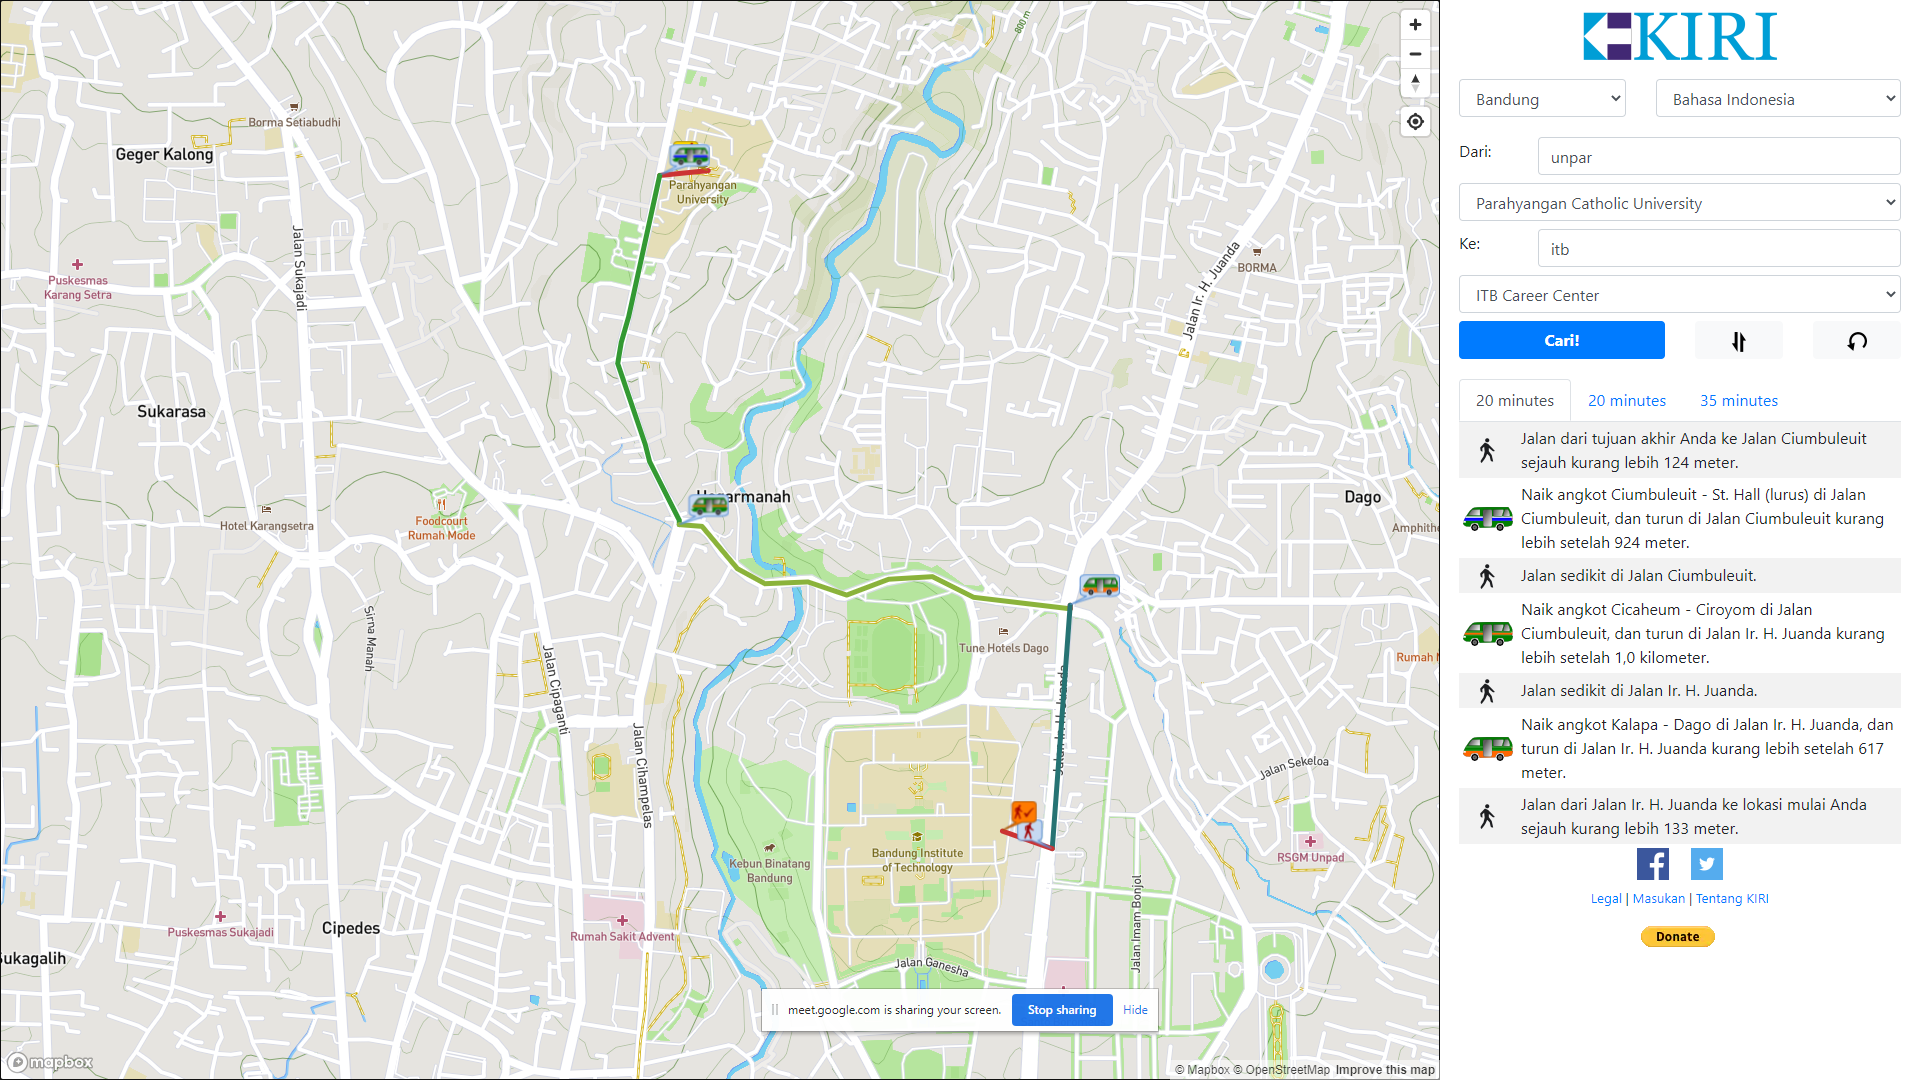
\includegraphics[scale=0.3]{Gambar/kiri-example-1}
    \caption{Tampilan utama website KIRI}
    \label{fig:my_label}
\end{figure}




\section{JSON}
\label{subsec:json}
JSON (\textit{JavaScript Object Notation}) adalah notasi berbasis teks,
   format pertukaran data bahasa-independen. berasal dari
   Standar Bahasa Pemrograman ECMAScript \cite{RFC:7159}. JSON merupakan format teks yang tidak bergantung pada bahasa pemprograman apapun karena menggunakan gaya bahasa yang umum digunakan oleh bahasa pemrograman C termasuk C, C++, C\#, Java, JavaScript, Perl, Python, dan lain-lain. Oleh karena sifat-sifat tersebut, menjadikan JSON ideal sebagai bahasa pertukaran-data. JSON memiliki enam tipe data, yaitu \textit{string}, angka, \textit{null}, \textit{array} (ditandai dengan tanda kurung siku ($\left [ \right ]$)), \textit{object} (ditandai dengan tanda kurung kurawal (\{\})), dan \textit{boolean} (\textit{true} dan \textit{false}). Struktur utama JSON terdiri dari pasangan nama atau nilai yang dipisahkan dengan tanda titik dua (:). Contoh struktur JSON mengenai tipe dan jenis atribut dapat dilihat pada Listing~ \ref{listing:JSON}.

\begin{lstlisting}[caption=Contoh Struktur JSON, label=listing:JSON]
 {
 "timestamp":"2014-1-2:0:11",
 "start":"-6.8972513,107.6385574",
 "finish":"-6.91358,107.62718"
 }
\end{lstlisting}

\section{CSV}
\label{subsec:csv}
CSV (\textit{Comma Separated Values}) adalah suatu format data dalam basis data di mana setiap nilai atribut dipisahkan dengan tanda koma (,) dan setiap baris data ditandai dengan baris baru.\cite{RFC:4180} CSV digunakan untuk bertukar data dan mengonversi data dari sebuah program \textit{spreadsheet} ke program \textit{spreadsheet} lainnya. Contoh CSV dapat dilihat pada Listing~\ref{listing:CSV}.

\begin{lstlisting}[caption=Contoh CSV, label=listing:CSV]
    logId,APIKey,Timestamp (UTC),Action,AdditionalData
    113909,E5D9904F0A8B4F99,2/1/2014 0:07,PAGELOAD,/5.10.83.30/
    113910,E5D9904F0A8B4F99,2/1/2014 0:07,PAGELOAD,/5.10.83.49/
\end{lstlisting}
	
\section{Google Maps Javascript API}
\label{sec:googlemaps}
Google Maps adalah layanan pemetaan web yang dikembangkan oleh Google. Menawarkan citra satelit, foto udara, dan peta jalan yang interaktif, kondisi lalu lintas secara \textit{real time} \cite{mehta:19:gmaps}.
 \begin{figure}[H]
    \centering
    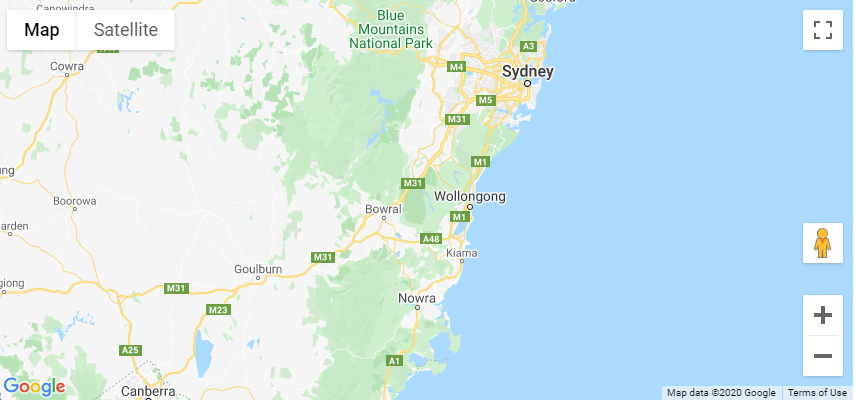
\includegraphics[scale=0.5]{Gambar/example_google_map.PNG}
    \caption{Contoh Heat Map }
    \label{fig:my_label}
\end{figure}
Google Maps dalam service nya telah menyediakan \textit{API (pplication programming interface)} yang dapat di gunakan untuk public.
aplication programming interface adalah \textit{computer interface} yang mengatur komunikasi antar perangkat lunak \cite{libby:20:api}.
Google Maps telah menyediakan beberapa teknik pemetaan data yaitu :
 \begin{itemize}
     \item \textit{Heat Map}
     \item \textit{Marker Clustering}

 \end{itemize}
 terdapat beberapa parmeter untuk menginisialisasi \textit{Google Maps Javascript API}
 \begin{itemize}
     \item \textit{Google Maps Object}
     \item \textit{Position}
     \item \textit{Zoom Level}
 \end{itemize}
 
 \subsection{\textit{Position}}
 \textit{Google Maps} menggunakan \textit{Latitude} dan \textit{Longitude}  sebagai atribute untuk menyatakan sebuah posisi.
 \textit{Latitude} adalah garis yang horisontal / mendatar. Titik 0 adalah sudut ekuator, tanda + menunjukan arah ke atas menuju kutub utara, sedangkan tanda minus di koordinat Latitude menuju ke kutub selatan. \textit{Longitude} adalah garis lintang . Angka dari sudut bundar bumi horisontal. Titik diawali dari 0 ke 180 derajat, dan 0 ke-180 ke arah sebaliknya.
 
 
 
 \subsection{\textit{Google Maps Object}}
 \textit{Maps Object} adalah Kelas \textit{JavaScript} yang mewakili peta adalah kelas Peta. Objek kelas ini mendefinisikan satu peta di halaman. (Anda dapat membuat lebih dari satu \textit{instance} kelas ini - setiap objek akan menentukan peta terpisah pada halaman.) Kami membuat \textit{instance} baru dari kelas ini menggunakan \textit{operator} baru \textit{JavaScript}.
  \begin{lstlisting}
    map = new google.maps.Map(document.getElementById("map"), {...});
 \end{lstlisting}
 \subsection{\textit{Heat Map}}
 \label{subsec:heat map}
 \textit{Heat Map} adalah sebuah teknik visualisasi data dimana data digambarkan sebagai warna. Saat Lapisan \textit{heat map} diaktifkan, hamparan berwarna akan muncul di atas map. Secara  \textit{default}, area dengan intensitas lebih tinggi akan diwarnai merah, dan area dengan intensitas lebih rendah akan tampak hijau.

 \begin{figure}[H]
    \centering
    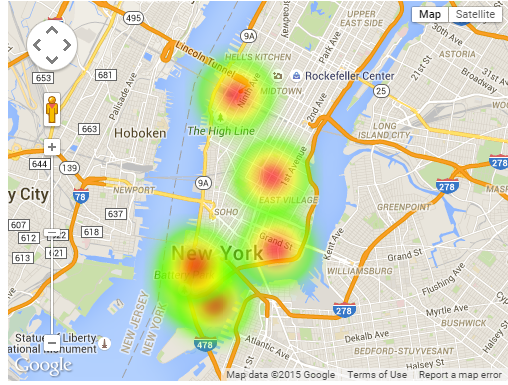
\includegraphics[scale=0.5]{Gambar/heat-map-example}
    \caption{Contoh Heat Map }
    \label{fig:my_label}
\end{figure}

Beberapa Jenis \textit{Heat Map}:
 \begin{itemize}
     \item \textit{Click-tracking map}
     \item \textit{Scroll map}
     \item \textit{Hover/Mouse tracking map}
     \item \textit{Eye tracking map}
 \end{itemize}
 
 Untuk menampilkan \textit{heat map } menggunakan \textit{Google Javascript API} dapat menggunakan syntax.
 \begin{lstlisting}
var heatmap = new google.maps.visualization.HeatmapLayer({
  data: heatMapData
});
heatmap.setMap(map);

\end{lstlisting}
 
 \subsection{\textit{Marker}}
 \label{subsec:heat map}
 \textit{Marker } adalah suatu tanda yang di pasang di dalam sebuah maps atau peta sebagai petanda lokasi atau tempat. Marker  dapat menampilkan gambar khusus, dalam hal ini biasanya disebut sebagai \textit{icon}.\cite{GoogleMarker:01:Maps}.
 Untuk Menambahkan Marker.Untuk menambahkan \textit{Marker} pada \textit{Google Map Javascript Api} membutuhkan beberapa parameter
  \begin{itemize}
     \item \textit{Position}  menggunakan latlng untuk mengidentifikasi letak suatu tempat
     \item \textit{Map} menggunakan object map dari google javascript api
 \end{itemize}
 \begin{figure}[H]
    \centering
    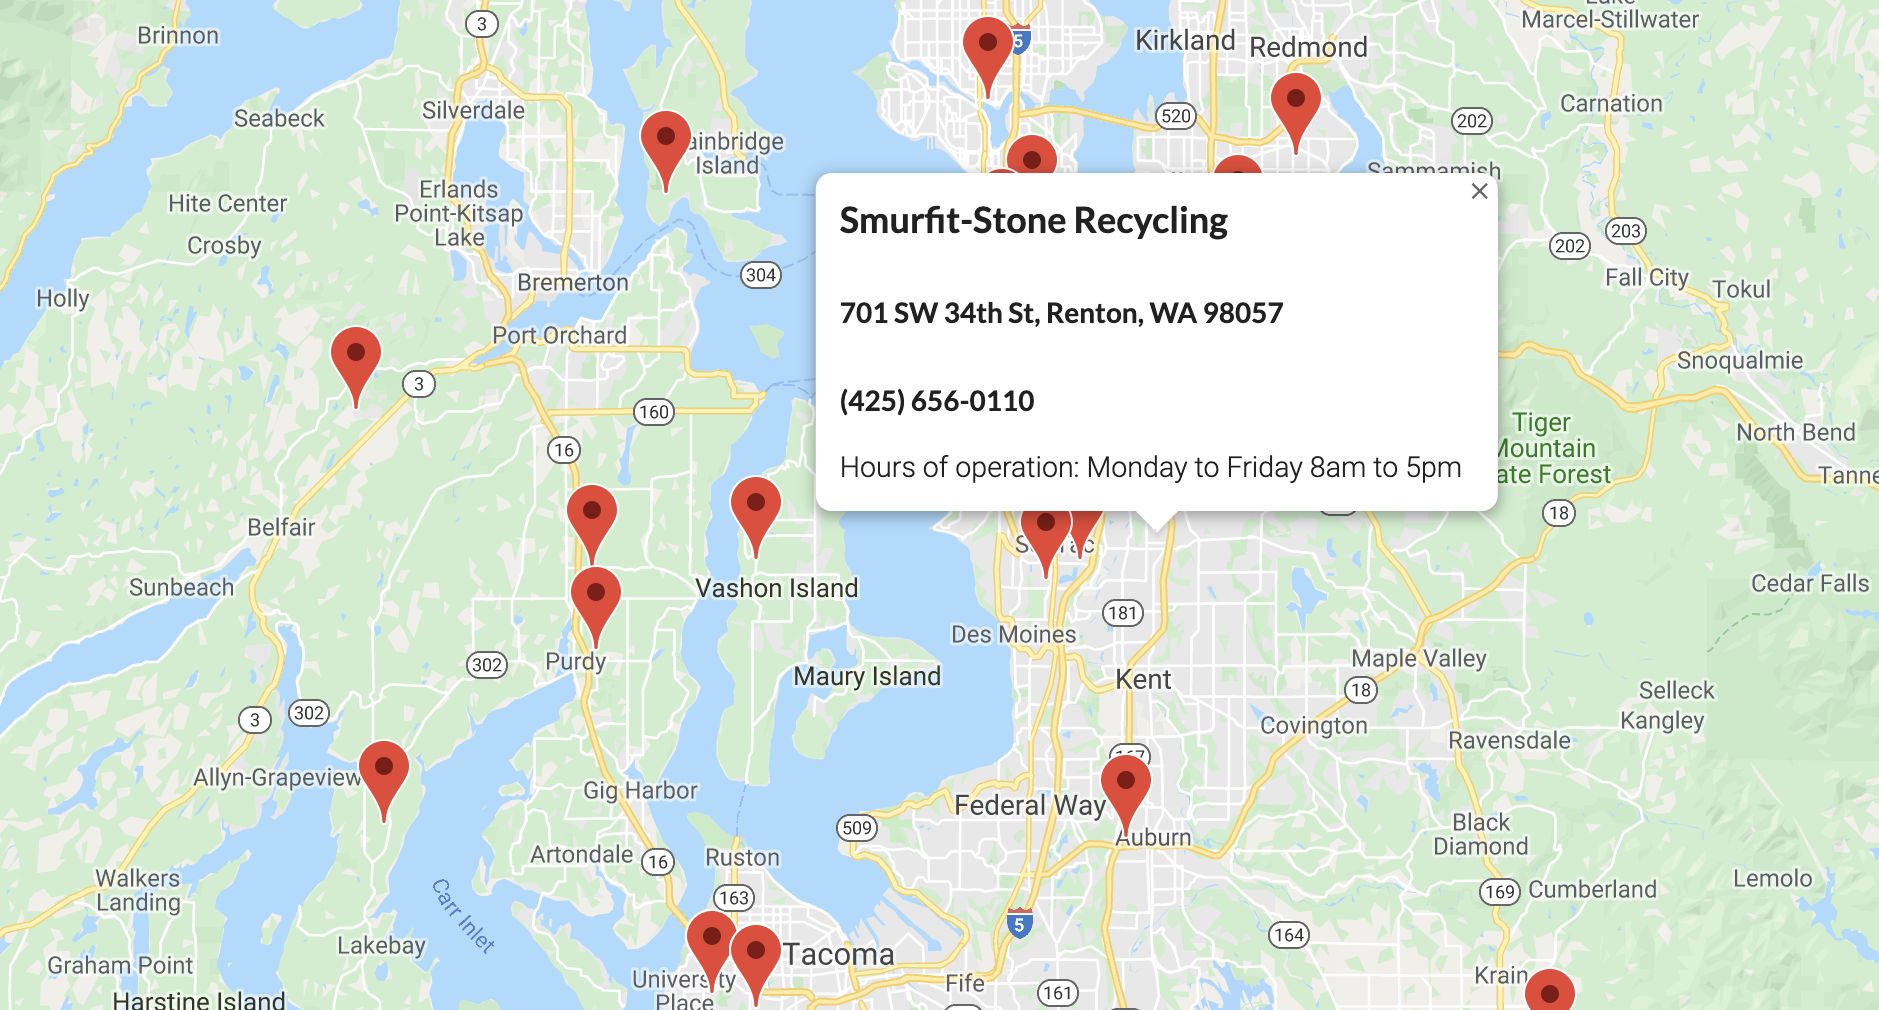
\includegraphics[scale=0.2]{Gambar/marker_example.png}
    \caption{Contoh Marker}
    \label{fig:my_label}
\end{figure}

Untuk menambahkan \textit{Marker} dapat menggunakan \textit{syntax} seperti:
\begin{lstlisting}
var heatmap = new google.maps.visualization.HeatmapLayer({
  data: heatmapData
});
heatmap.setMap(map);

\end{lstlisting}
  \begin{figure}[H]
    \centering
    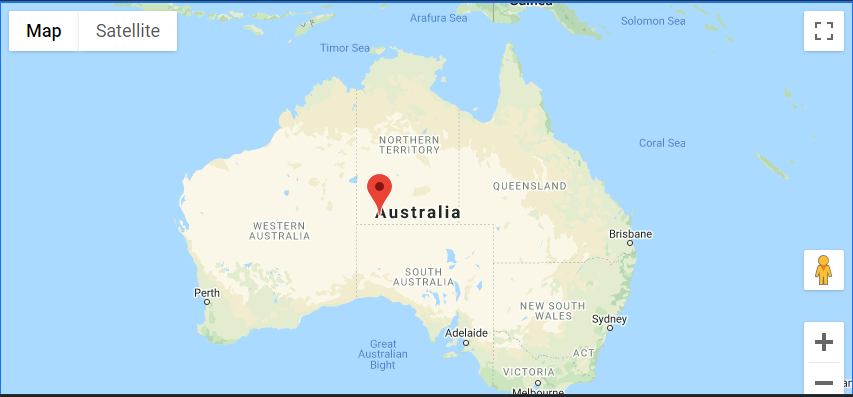
\includegraphics[scale=0.5]{Gambar/add_marker.PNG}
    \caption{Add Marker}
    \label{fig:my_label}
\end{figure}




 
\section{\textit{Marker Clustering}}
 \textit{Marker Clustering } adalah teknik visualisasi data dimana data akan di representasikan sebagai tanda / \textit{Mark} pada suatu space 2 dimensi, semakin banyak data yang terdapat pada suatu tempat maka akan semakin banyak quantitas penanda / \textit{Mark} yang di berikan. \cite{GoogleMarkerCluster:01:Maps}
  \begin{figure}[H]
    \centering
    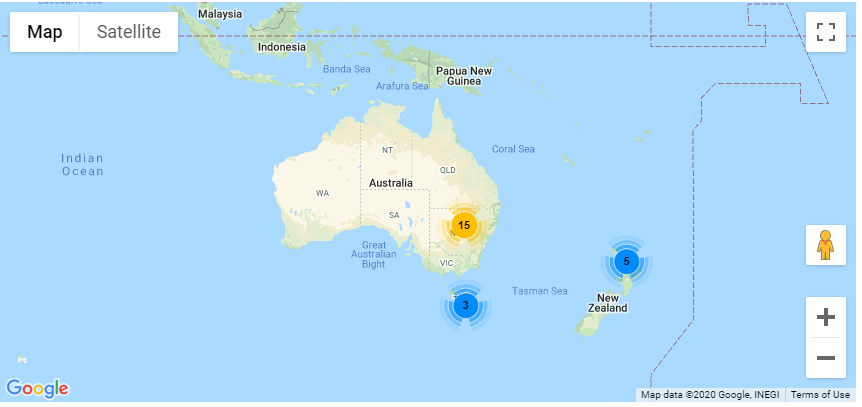
\includegraphics[scale=0.5]{Gambar/marker_clustering.PNG}
    \caption{Contoh Marker Clustering}
    \label{fig:my_label}
\end{figure}
Untuk menggunakan \textit{Marker Clustering} pada \textit{Google Maps Javascript API} dapat menggunakan Object \textit{Marker Clusterer} yang telah di sediakan oleh \textit{Google Maps} 
  \begin{lstlisting}
  new MarkerClusterer(map, markers, {
    imagePath:
      "https://developers.google.com/maps/documentation/javascript/examples/markerclusterer/m",
  });
}
 \end{lstlisting}
 \textit{Marker Clustering} akan menggunakan   \textit{grid-based clustering technique} yang membagi peta menjadi kotak dengan ukuran tertentu (ukuran berubah di setiap tingkat zoom), dan mengelompokkan penanda ke dalam setiap kisi persegi. Ini membuat \textit{cluster} di \textit{marker} tertentu, dan menambahkan marker yang berada dalam batas-batasnya ke \textit{cluster}.\textit{Marker Clustering} merupakan sebuah teknik yang menggunakan \textit{Marker} sehingga untuk dapat memunculkan \textit{Marker Clustering} diperlukan object \textit{Marker}
 berikut ini contoh pengimplenentasian \textit{Marker Clustering} 
 
 \begin{lstlisting}
function initMap() {
  const map = new google.maps.Map(document.getElementById("map"), {
    zoom: 3,
    center: { lat: -28.024, lng: 140.887 },
  });
  const labels = "ABCDEFGHIJKLMNOPQRSTUVWXYZ";
  const markers = locations.map((location, i) => {
    return new google.maps.Marker({
      position: location,
      label: labels[i % labels.length],
    });
  });
  new MarkerClusterer(map, markers, {
    imagePath:"",
  });
}
const locations = [
  { lat: -31.56391, lng: 147.154312 },
  { lat: -33.718234, lng: 150.363181 },
  { lat: -33.727111, lng: 150.371124 },
];
\end{lstlisting}